%************************************************
\chapter[Appendix 4: Chapter 4 - Supplementary materials]{Appendix 4: Chapter 4 - Supplementary materials}\label{ch:POLS_appendix}
%************************************************
\renewcommand{\thefigure}{A.4.\arabic{figure}}
\setcounter{figure}{0}

\renewcommand{\thetable}{A.4.\arabic{table}}
\setcounter{table}{0}

\section*{Supplementary tables}

\begin{table}[ht!]
\centering
\caption[Intra-class correlation coefficients]{
Gaussian BPMMs used to estimate intra-class correlation coefficients for
variation in FID (log-transformed).}\label{tab:tabApp4.1}
\begin{tabular}{llllll}
\toprule
\multicolumn{6}{@{}l@{}}{\textbf{Model for all observations (n = 11,852 observations of 317 species)}}        \\
\midrule
             & \textbf{post mean} & \textbf{L-95\% CI} & \textbf{U-95\%} & \textbf{eff.samp} & \textbf{pMCMC} \\
\multicolumn{6}{@{}l@{}}{\textbf{Random effects}}                                                   \\
Phylogeny            & 0.299          & 0.172          & 0.451    & 1000       & -                  \\
Species              & 0.222          & 0.163          & 0.274    & 890.6      & -                  \\
Residual             & 0.263          & 0.256          & 0.269    & 1151       & -                  \\
\multicolumn{6}{@{}l@{}}{\textbf{Fixed effects}}                                                    \\
Intercept            & 3.238          & 2.780          & 3.675    & 1000       & \textless{0.001}   \\
\noalign{\bigskip}
\toprule
\multicolumn{6}{@{}l@{}}{\textbf{Model for rural observations (n = 7,373 observations of 303 species)}}       \\
\midrule
             & \textbf{post mean} & \textbf{L-95\% CI} & \textbf{U-95\%} & \textbf{eff.samp} & \textbf{pMCMC} \\
\multicolumn{6}{@{}l@{}}{\textbf{Random effects}}                                                   \\
Phylogeny            & 0.316          & 0.178          & 0.465    & 1000       & -                  \\
Species              & 0.187          & 0.135          & 0.247    & 1585       & -                  \\
Residual             & 0.230          & 0.223          & 0.238    & 638.2      & -                  \\
\multicolumn{6}{@{}l@{}}{\textbf{Fixed effects}}                                                    \\
Intercept            & 3.348          & 2.924          & 3.801    & 1201       & \textless{0.001}   \\
\noalign{\bigskip}
\toprule
\multicolumn{6}{@{}l@{}}{\textbf{Model for urban observations (n = 4479 observations of 108 species)}}        \\
\midrule
             & \textbf{post mean} & \textbf{L-95\% CI} & \textbf{U-95\%} & \textbf{eff.samp} & \textbf{pMCMC} \\
\multicolumn{6}{@{}l@{}}{\textbf{Random effects}}                                                   \\
Phylogeny            & 0.249          & 0.065          & 0.477    & 1000       & -                  \\
Species              & 0.127          & 0.055          & 0.215    & 1000       & -                  \\
Residual             & 0.173          & 0.166          & 0.180    & 1000       & -                  \\
\multicolumn{6}{@{}l@{}}{\textbf{Fixed effects}}                                                    \\
Intercept            & 2.491          & 2.050          & 2.955    & 1000       & \textless{0.001}
\end{tabular}
\end{table}


\begin{table}
\centering
\caption[Best FID models for areas with rural and urban observations]{
Gaussian BPMMs accounting for variation in FID (log-transformed) as a
function of habitat, based on information from regions for which both urban and
rural FID observations were available (Denmark, France, Norway and China). The
model below includes only species for which FIDs were recorded for both urban
and rural habitats.}\label{tab:tabApp4.2}
\begin{tabular}{llllll}
\toprule
\multicolumn{6}{@{}l@{}}{\textbf{Model for all observations (n = 11,852 observations of 317 species)}}     \\
\midrule
          & \textbf{post mean} & \textbf{L-95\% CI} & \textbf{U-95\%} & \textbf{eff.samp} & \textbf{pMCMC} \\
\multicolumn{6}{@{}l@{}}{\textbf{Random effects}}                                         \\
Phylogeny         & 0.424        & 0.205        & 0.656  & 871      & -                   \\
Species           & 0.132        & 0.064        & 0.192  & 1000     & -                   \\
Country           & 0.133        & 0.011        & 0.459  & 1000     & -                   \\
Residual          & 0.204        & 0.198        & 0.209  & 1000     & -                   \\
\multicolumn{6}{@{}l@{}}{\textbf{Fixed effects}}                                          \\
Intercept         & 3.069        & 2.519        & 3.719  & 1000     & \textless{0.001}    \\
Habitat:urban     & -0.397       & -0.417       & -0.377 & 1222     & \textless{0.001}    \\
Height            & 0.017        & 0.014        & 0.020  & 1000     & \textless{0.001}    \\
\noalign{\bigskip}
\toprule
\multicolumn{6}{@{}l@{}}{\textbf{Model for species present in both urban and rural habitats (9266 observations of 246 species)}} \\
\midrule
          & \textbf{post mean} & \textbf{L-95\% CI} & \textbf{U-95\%} & \textbf{eff.samp} & \textbf{pMCMC} \\
\multicolumn{6}{@{}l@{}}{\textbf{Random effects}}                                          \\
Phylogeny         & 0.204        & 0.080        & 0.346  & 1000     & -                    \\
Species           & 0.098        & 0.050        & 0.151  & 1000     & -                    \\
Country           & 0.174        & 0.010        & 0.513  & 596      & -                    \\
Residual          & 0.204        & 0.198        & 0.209  & 1093     & -                    \\
\multicolumn{6}{@{}l@{}}{\textbf{Fixed effects}}                                           \\
Intercept         & 2.854        & 2.343        & 3.415  & 1182     & \textless{0.001}     \\
Habitat:urban     & -0.400       & -0.423       & -0.380 & 906      & \textless{0.001}     \\
Height            & 0.016        & 0.013        & 0.020  & 1000     & \textless{0.001}
\end{tabular}
\end{table}


\begin{table}
\centering
\caption[Best FID models]{Gaussian BPMM accounting for variation in FID 
(log-transformed) as a
function of the fast-slow continuum, based on information from all regions
(11,392 observations belonging to 246 species).}\label{tab:tabApp4.3}
\begin{tabular}{lllllllllll}
\toprule
        & \textbf{post mean} & \textbf{L-95\% CI} & \textbf{U-95\%} & \textbf{eff.samp} & \textbf{pMCMC} \\
\multicolumn{6}{@{}l@{}}{\textbf{Random effects}}                                          \\
Animal             & 0.238         & 0.118        & 0.358  & 1791     & -                  \\
Species            & 0.153         & 0.103        & 0.202  & 1000     & -                  \\
Country            & 0.113         & 0.020        & 0.307  & 1118     & -                  \\
Residual           & 0.209         & 0.204        & 0.214  & 1000     & -                  \\
\multicolumn{6}{@{}l@{}}{\textbf{Fixed effects}}                                           \\
Intercept          & 3.192         & 2.694        & 3.655  & 1000     & \textless{0.001}   \\
FS                 & 0.019         & 0.008        & 0.030  & 1074     & \textless{0.001}   \\
Habitat:urban      & -0.403        & -0.424       & -0.382 & 1000     & \textless{0.001}   \\
Height             & 0.014         & 0.011        & 0.017  & 1000     & \textless{0.001}
\end{tabular}
\end{table}


\begin{table}
\caption[FID model with brain size for rural habitats]{Gaussian BPMM accounting 
for variation in FID (log-transformed) in
rural habitats as a function of residual brain size, based on information from
all regions (3297 observations of 105 species). We restricted the analysis to
rural habitats as previous work suggests that large-brained birds are
over-represented in urbanised environments.}\label{tab:tabApp4.4}
\begin{tabular}{llllll}
\toprule
                    & \textbf{post mean} & \textbf{L-95\% CI} & \textbf{U-95\%} & \textbf{eff.samp} & \textbf{pMCMC} \\
\multicolumn{6}{@{}l@{}}{\textbf{Random effects}}                                          \\
Phylogeny           & 0.290          & 0.136        & 0.480  & 1000     & -                \\
Species             & 0.112          & 0.051        & 0.174  & 1000     & -                \\
Residual            & 0.242          & 0.231        & 0.253  & 1000     & -                \\
\multicolumn{6}{@{}l@{}}{\textbf{Fixed effects}}                                           \\
Intercept           & 3.135          & 2.701        & 3.635  & 827.9    & \textless{0.001} \\
Brain residual      & 0.667          & 0.260        & 1.132  & 1020.6   & 0.008            \\
Height              & 0.010          & 0.003        & 0.017  & 1000     & 0.014
\end{tabular}
\end{table}


\begin{table}
\caption[FID model with brain size for species in rural and urban habitats]{
Gaussian BPMM accounting for across species differences in FID from rural and
urban habitats (response variable) as a function of residual brain size, based
on information from species for which both urban and rural FID observations
were available. The decline of each species was estimated as the log(mean
FIDrural)- log(mean FIDurban). The model was repeated again restricting
the species to those with at least 15 FID observations in each habitat. The
models were run with a Gaussian structure of the errors and non-informative
priors. We weighted the observations by 1/( n-3), being “n” the number of FID
observations of the species.}\label{tab:tabApp4.5}
\begin{tabular}{llllll}
\toprule
\multicolumn{6}{@{}l@{}}{\textbf{Model for all observation (71 species)}}                                  \\
\midrule
          & \textbf{post mean} & \textbf{L-95\% CI} & \textbf{U-95\%} & \textbf{eff.samp} & \textbf{pMCMC} \\
\multicolumn{6}{@{}l@{}}{\textbf{Random effects}}                                                \\
Phylogeny           & 0.228             & 0.085          & 0.390    & 975        & -             \\
Residual            & 0.040             & 0.007          & 0.082    & 975        & -             \\
\multicolumn{6}{@{}l@{}}{\textbf{Fixed effects}}                                                 \\
Intercept           & 0.837             & 0.429          & 1.300    & 975        & 0.002         \\
Brain residual      & 0.160             & -0.296         & 0.694    & 975        & 0.545         \\
\noalign{\bigskip}
\toprule
\multicolumn{6}{@{}l@{}}{\textbf{Model with  species with at least 15 FID observations per hábitat (34 species)}} \\
\midrule
            & \textbf{post mean} & \textbf{L-95\% CI} & \textbf{U-95\%} & \textbf{eff.samp} & \textbf{pMCMC}      \\
\multicolumn{6}{@{}l@{}}{\textbf{Random effects}}                                                     \\
Phylogeny           & 0.154             & 0.059          & 0.258    & 975        & -                  \\
Residual            & 0.010             & 0.000          & 0.027    & 975        & -                  \\
\multicolumn{6}{@{}l@{}}{\textbf{Fixed effects}}                                                      \\
Intercept           & 0.867             & 0.471          & 1.281    & 975        & \textless{0.001}   \\
Brain residual      & 0.162             & -0.315         & 0.690    & 975        & 0.539
\end{tabular}
\end{table}
\clearpage

\section*{Supplementary figures}

\begin{figure}[ht!]
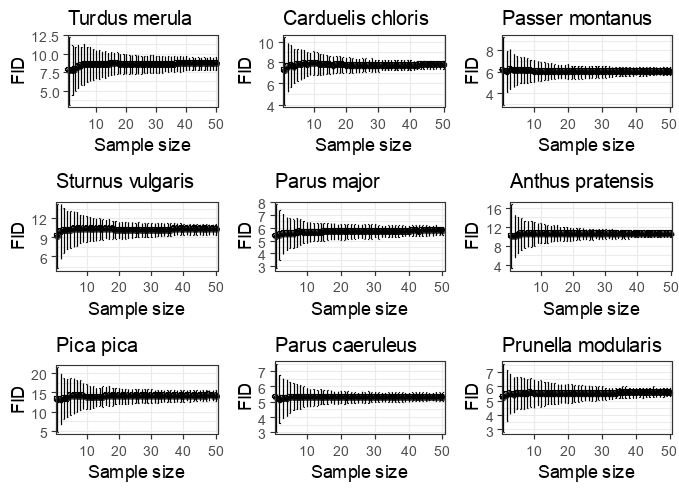
\includegraphics[width=\textwidth]{./Figures/Appendix4_1/Fig_1.png}
\caption[Effects of the sample size on FID estimates]{
Simulations to estimate the minimum sample size needed to accurately estimate
FID. See main text for details.}\label{fig:figApp4.1}
\end{figure}


\begin{figure}
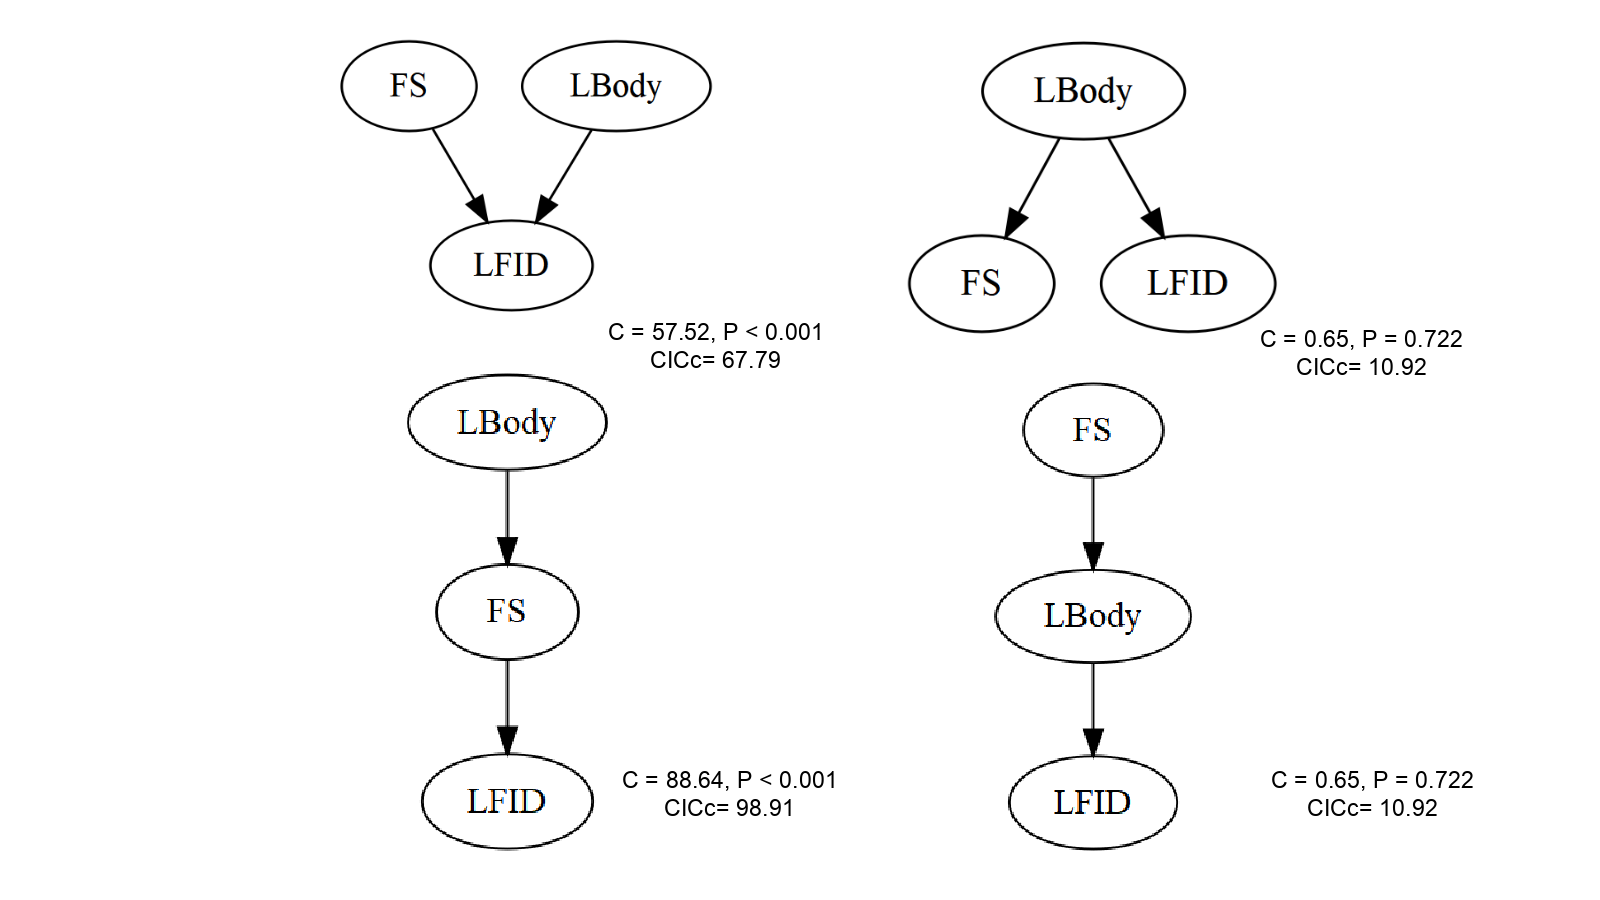
\includegraphics[width=\textwidth]{./Figures/Appendix4_1/Fig_2.png}
\caption[Path analysis with body size for rural habitats]{
Path diagrams of the causal scenarios analysed to study how body size affects
the relationship between flight initiation distance (FID) and the fast-slow
continuum (FS) in rural habitats. The letter “L” before body and FID
denotes log-transformation.}\label{fig:figApp4.2}
\end{figure}


\begin{figure}
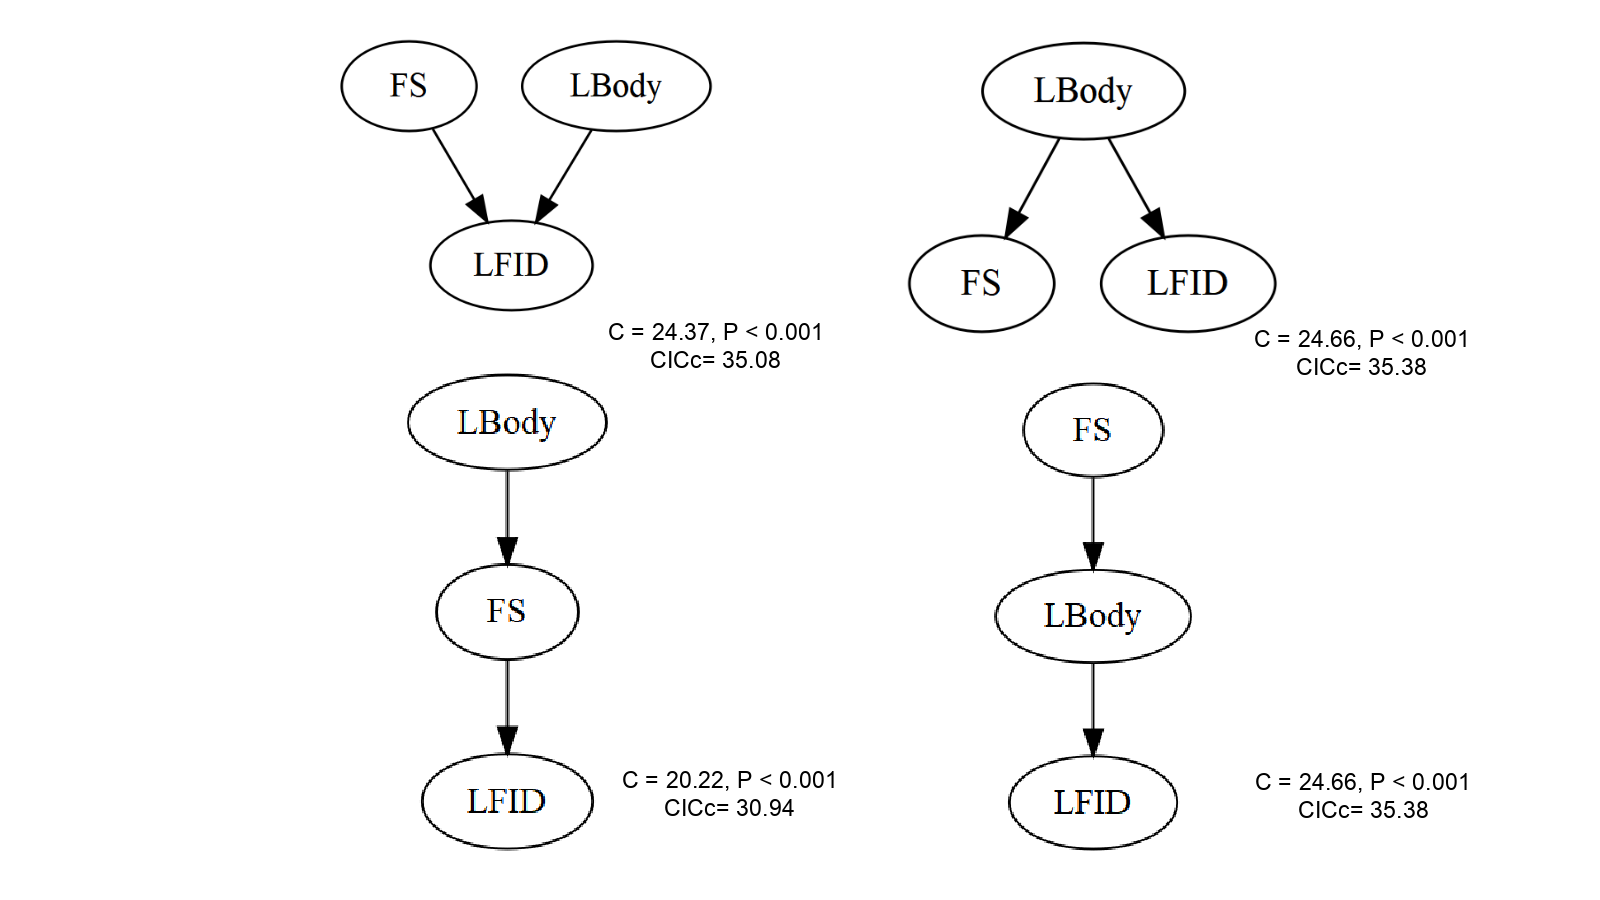
\includegraphics[width=\textwidth]{./Figures/Appendix4_1/Fig_3.png}
\caption[Path analysis with body size for urban habitats]{
Path diagrams of the causal scenarios analysed to study how body size affects
the FID-FS association in urban habitats. The letter “L” before body and
FID denotes log-transformation.}\label{fig:figApp4.3}
\end{figure}
